%worksheet5.tex
%problem set for the course Algorithms COMS10007 
%taught at the University of Bristol
%Conor Houghton conor.houghton@bristol.ac.uk

%To the extent possible under law, the author has dedicated all copyright 
%and related and neighboring rights to these notes to the public domain 
%worldwide. These notes are distributed without any warranty. 



\documentclass[11pt,a4paper]{scrartcl}
\typearea{12}
\usepackage{graphicx}
\usepackage{pstricks}
\usepackage{tikz-qtree}
\usepackage{listings}
\usepackage{color}

\newif\ifanswers
\answerstrue
%\answersfalse


\lstset{language=C}
\pagestyle{headings}
\markright{COMS10007 - algorithms worksheet 5 - Conor}
\begin{document}

\subsection*{Algorithms Worksheet 5}

This week there are four question worth two marks each, there are two
marks for attendance.

\begin{enumerate}

\item This is a question about AVL trees.  Add \lq{}1\rq{} to this tree and balance it.
\begin{center}
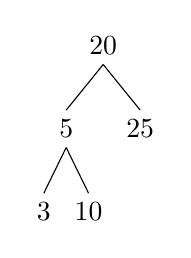
\begin{tikzpicture}
\Tree [.20 [.5 3 10 ] 25 ]
\end{tikzpicture}
\end{center}

\ifanswers

\noindent Solution:
So start with
\begin{center}
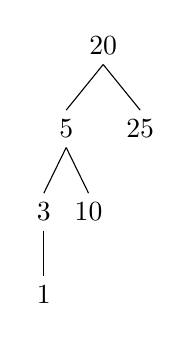
\begin{tikzpicture}
\Tree [.20 [.5 [.3 1 ] 10 ] 25 ]
\end{tikzpicture}
\end{center}
Clearly we need to rotate so that the \lq{}5\rq{} is on top but to do this the \lq{}10\rq{} has to move to the \lq{}25\rq{}:
\begin{center}
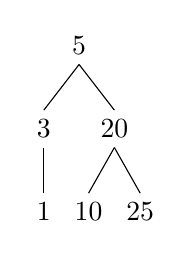
\begin{tikzpicture}
\Tree [.5 [.3 1 ] [.20 10 25 ] ]
\end{tikzpicture}
\end{center}

\fi

\item This is also a question about AVL trees.  Add \lq{}12\rq{} to this tree and balance it.
\begin{center}
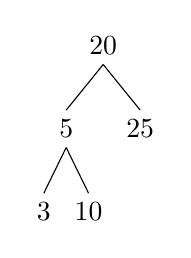
\begin{tikzpicture}
\Tree [.20 [.5 3 10 ] 25 ]
\end{tikzpicture}
\end{center}

\ifanswers

\noindent Solution:
So start with
\begin{center}
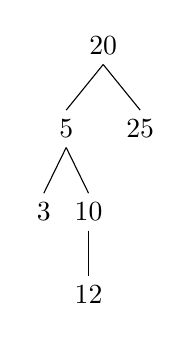
\begin{tikzpicture}
\Tree [.20 [.5 3 [.10 12 ] ] 25 ]
\end{tikzpicture}
\end{center}
Clearly we need to rotate so that the \lq{}10\rq{} is on top but to do this the \lq{}12\rq{} has to move to the \lq{}25\rq{}:
\begin{center}
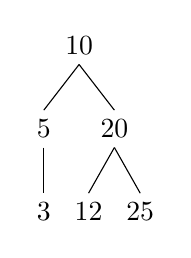
\begin{tikzpicture}
\Tree [.10 [.5 3 ] [.20 12 25 ] ]
\end{tikzpicture}
\end{center}

\fi




\item  Heapify the list $(15,2,23,19,24,13,8)$.

\ifanswers

\noindent Solution: The key point is you add each item at the next
available slot in the tree and then if it violates the rule that items are smaller than their parent, you swap it upwards until it works. So
\begin{center}
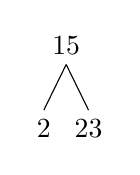
\begin{tikzpicture}
\Tree [.15 2 23 ]
\end{tikzpicture}
\end{center}
gets changed to
\begin{center}
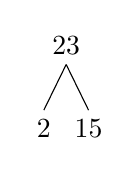
\begin{tikzpicture}
\Tree [.23 2 15 ]
\end{tikzpicture}
\end{center}
Next adding to the next layer
\begin{center}
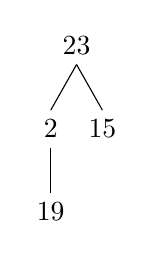
\begin{tikzpicture}
\Tree [.23 [.2 19 ] 15 ]
\end{tikzpicture}
\end{center}
becomes
\begin{center}
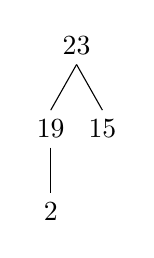
\begin{tikzpicture}
\Tree [.23 [.19 2 ] 15 ]
\end{tikzpicture}
\end{center}
and then
\begin{center}
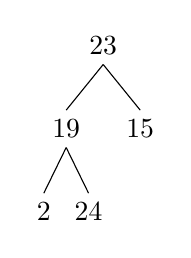
\begin{tikzpicture}
\Tree [.23 [.19 2 24 ] 15 ]
\end{tikzpicture}
\end{center}
goes to
\begin{center}
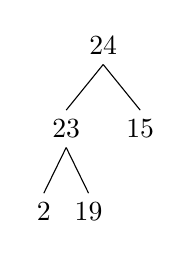
\begin{tikzpicture}
\Tree [.24 [.23 2 19 ] 15 ]
\end{tikzpicture}
\end{center}
Next
\begin{center}
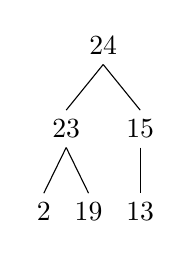
\begin{tikzpicture}
\Tree [.24 [.23 2 19 ] [.15 13 ] ]
\end{tikzpicture}
\end{center}
becomes
\begin{center}
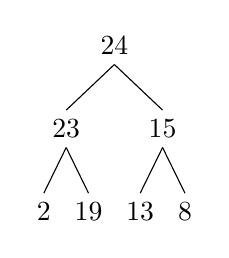
\begin{tikzpicture}
\Tree [.24 [.23 2 19 ] [.15 13 8 ] ]
\end{tikzpicture}
\end{center}
and then it finishes.
\fi

\item For the heap
\begin{center}
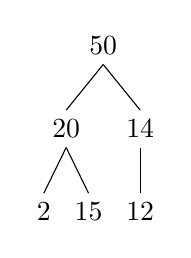
\begin{tikzpicture}
\Tree [.50 [.20 2 15 ] [.14 12  ] ]
\end{tikzpicture}
\end{center}
remove the top element and restore the heap property.


\ifanswers

\noindent Solution. First you swap the last element to the top and remove the old top element:
\begin{center}
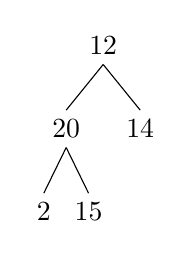
\begin{tikzpicture}
\Tree [.12 [.20 2 15 ] [.14  ] ]
\end{tikzpicture}
\end{center}
then you push the top element down by swapping it with the larger of its children until it can't go down further:
\begin{center}
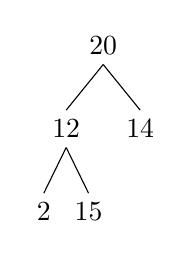
\begin{tikzpicture}
\Tree [.20 [.12 2 15 ] [.14  ] ]
\end{tikzpicture}
\end{center}
and
\begin{center}
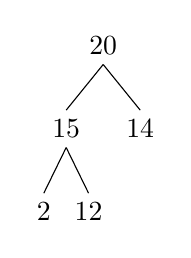
\begin{tikzpicture}
\Tree [.20 [.15 2 12 ] [.14  ] ]
\end{tikzpicture}
\end{center}
\fi
\end{enumerate}
\end{document}
